% This file was created with tikzplotlib v0.10.1.
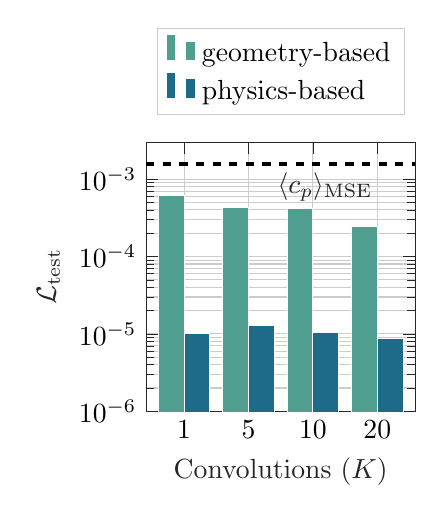
\begin{tikzpicture}

\definecolor{cadetblue79158143}{RGB}{79,158,143}
\definecolor{darkslategray38}{RGB}{38,38,38}
\definecolor{lightgray204}{RGB}{204,204,204}
\definecolor{teal29107137}{RGB}{29,107,137}

\begin{axis}[
width=5cm,
height=5cm,
% font=\footnotesize,
axis line style={darkslategray38},
legend cell align={left},
legend columns=1,
legend style={
  fill opacity=1,
  draw opacity=1,
  text opacity=1,
  at={(0.5,1.1)},
  anchor=south,
  draw=lightgray204,
  % column sep = 0.1cm
},
log basis y={10},
tick align=inside,
x grid style={lightgray204},
xlabel=\textcolor{darkslategray38}{Convolutions (\(\displaystyle K\))},
xmajorgrids,
xmajorticks=true,
xmin=-0.59, xmax=3.59,
% xminorgrids,
xtick style={color=darkslategray38},
xtick={0,1,2,3},
xticklabels={$1$,$5$,$10$,$20$},
y grid style={lightgray204},
ylabel=\textcolor{darkslategray38}{\(\displaystyle \mathcal{L}_{\mathrm{test}}\)},
ymajorgrids,
ymajorticks=true,
% ymin=6.65631281836172e-06, ymax=0.003,
% ymin=1.59801652953767e-06, ymax=0.003,
yminorgrids,
ymode=log,
ytick style={color=darkslategray38},
ymin=1e-06, ymax=0.003,
    ymode=log,
    ytick style={color=darkslategray38},
]

\def\epsVal{1e-8}

\draw[draw=white,fill=cadetblue79158143] (axis cs:-0.4,\epsVal) rectangle (axis cs:0,0.00060891);

\addlegendimage{ybar,ybar legend,draw=white,fill=cadetblue79158143, legend image post style={xscale=1.2,yscale=1.2}}
% \addlegendentry{GBF}
\addlegendentry{geometry-based}

\draw[draw=white,fill=cadetblue79158143] (axis cs:0.6,\epsVal) rectangle (axis cs:1,0.00043075);
\draw[draw=white,fill=cadetblue79158143] (axis cs:1.6,\epsVal) rectangle (axis cs:2,0.00042087);
\draw[draw=white,fill=cadetblue79158143] (axis cs:2.6,\epsVal) rectangle (axis cs:3,0.00024596);
\draw[draw=white,fill=teal29107137] (axis cs:-2.77555756156289e-17,\epsVal) rectangle (axis cs:0.4,1.01483165e-05);
\addlegendimage{ybar,ybar legend,draw=white,fill=teal29107137, legend image post style={xscale=1.2,yscale=1.2}}
% \addlegendentry{PBF}
\addlegendentry{physics-based}

\draw[draw=white,fill=teal29107137] (axis cs:1,\epsVal) rectangle (axis cs:1.4,1.28008924e-05);
\draw[draw=white,fill=teal29107137] (axis cs:2,\epsVal) rectangle (axis cs:2.4,1.04925812e-05);
\draw[draw=white,fill=teal29107137] (axis cs:3,\epsVal) rectangle (axis cs:3.4,8.63228706e-06);

\addplot [line width = 1.5pt, dashed, black]%, forget plot]
table {
-0.59 0.00156303563624041
3.59 0.00156303563624041
};
% \draw (axis cs:2.6,0.82) node[
%   scale=1,
%   anchor=west,
%   text=darkslategray38,
%   rotate=0.0
% ]{$ \langle c_p \rangle _ {\mathrm{MSE}}$};

\draw (axis cs:1.3,0.0008) node[
  scale=1,
  anchor=west,
  text=darkslategray38
]{$ \langle c_p \rangle _ {\mathrm{MSE}}$};


\end{axis}

\end{tikzpicture}
